\documentclass[10pt, fleqn]{article}
\usepackage[a4paper,margin=0.5in]{geometry}
\usepackage{multicol}
\usepackage{amsmath, amssymb}
\usepackage{titlesec}
\usepackage{float}
\usepackage{amsfonts, bm, graphicx}
\usepackage{enumitem}
\usepackage[font=small, skip=4pt]{caption}

\setlength{\abovedisplayskip}{6pt}
\setlength{\belowdisplayskip}{6pt}
\setlength{\abovedisplayshortskip}{4pt}
\setlength{\belowdisplayshortskip}{4pt}

\setlength{\textfloatsep}{8pt plus 2pt minus 2pt}
\setlength{\intextsep}{6pt plus 2pt minus 2pt}
\setlength{\floatsep}{8pt plus 2pt minus 2pt}

\setlength{\mathindent}{0pt}

\titleformat{\section}{\large\bfseries}{}{0em}{}
\titleformat{\subsection}{\normalsize\bfseries}{}{0em}{}
% Uppercase Volume with thicker, higher line
\newcommand{\vol}{\mathord{\text{\ooalign{\hidewidth $V$\hidewidth\cr\kern-0.5pt\raisebox{0.8ex}{\rule[0pt]{1em}{0.5pt}}}}}}

% Lowercase Volume with built-in shifts
\newcommand{\svol}{%
  \mathord{\text{\ooalign{%
    \hfil$v$\hfil\cr
    \hfil\rule[0.6ex]{0.8em}{0.5pt}\hfil
  }}}%
}
\begin{document}

\begin{center}
    \Large \textbf{Thermodynamics Formula Sheet} \\
    \normalsize Final Exam
\end{center}
    \section*{Units and Conversions}
    \vspace{-1em}
\begin{multicols}{2}\noindent
\textbf{SI Prefixes}
\makeatletter
\@fleqnfalse
\makeatother
\[
\begin{array}{ll@{\qquad}ll}
\text{femto (f)} &= 10^{-15} & \text{deca (da)} &= 10^{1} \\
\text{pico (p)} &= 10^{-12} & \text{hecto (h)} &= 10^{2} \\
\text{nano (n)} &= 10^{-9}  & \text{kilo (k)} &= 10^{3} \\
\text{micro ($\mu$)} &= 10^{-6} & \text{mega (M)} &= 10^{6} \\
\text{milli (m)} &= 10^{-3} & \text{giga (G)} &= 10^{9} \\
\text{centi (c)} &= 10^{-2} & \text{tera (T)} &= 10^{12} \\
\text{deci (d)} &= 10^{-1}  & \text{peta (P)} &= 10^{15}
\end{array}
\]
\makeatletter
\@fleqntrue
\makeatother
\textbf{Atmospheric Pressure}
\begin{flalign*}
1 \text{ atm} &= 101.325 \text{ kPa} &&= 29.92 \text{ inHg} & \\
&= 1.01325 \text{ bar} &&= 14.696 \text{ psi} & \\
&= 760 \text{ Torr} &&= 10.33 \text{ m H}_2\text{O (at 4$^\circ$C)} & \\
&= 760 \text{ mmHg} && &
\end{flalign*}
\textbf{Pressure Conversions}
\[1\,\text{Pa} = 1\,\text{N/m}^2\]
\[1\, \text{ bar} = 10^{5}\, \text{ Pa}\]
\[1\, \text{ psi} = 6.89476 \times 10^{3}\, \text{ Pa}\]
\[1\, \text{ Torr} = 133.322\, \text{ Pa}\]
\[1\, \text{ mmHg} = 133.322\, \text{ Pa}\]
\[1\, \text{ inHg} = 3.38639 \times 10^{3}\, \text{ Pa}\]
\textbf{Gauge vs Absolute Pressure}
\[P_{\text{gauge}} = P_{\text{absolute}} - P_{\text{atmospheric}}\]
\[P_{\text{vacuum}} = P_{\text{atmospheric}} - P_{\text{absolute}}\]
\underline{Note:} Generally, gauge pressures already account for atmospheric pressure, and thus reads zero when open to the atmosphere.\\
\textbf{Pressure Relations}
\[P = \frac{F}{A} = \rho g h \quad \text{(hydrostatic pressure)}\]
\[P_1 = P_2 \quad \Rightarrow \quad \frac{F_1}{A_1} = \frac{F_2}{A_2} \quad \text{(Pascal's Law)}\]
\[\Delta P = \rho g h \quad \text{(multi-fluid manometer)}\]
(add downward, subtract upward)\\\\
\textbf{Density and Specific Gravity}
\[\rho = \frac{m}{\vol}\quad \text{(density)}, \quad \svol = \frac{1}{\rho} = \frac{\vol}{m}  \quad \text{(specific volume)}\]
\textbf{Specific gravity} is defined as a relative density compared to water (at 4$^\circ$C) where $\rho_{water} = 1000\,\text{kg/m}^3$:
\[\text{SG} = \frac{\rho_{fluid}}{\rho_{water}} \implies \rho_{fluid} = SG \cdot \rho_{water}\]
\textbf{Specific Weight}
\[\gamma_s = \rho g \quad \text{(specific weight)}\]
Where hydrostatic pressure can be written as $P = \gamma_s h$
\newcolumn\\
\textbf{Multi-fluid Manometer}
\begin{enumerate}
    \item Begin at a known pressure point (gauge or atmospheric pressure) and follow the fluid layers to the unknown pressure point.
    \item Sign convention: add when going down, subtract when going up.
    \item \textbf{Horizontal jump:} We can "jump" horizontally across bends in the tube if both sides of the jump are within the \textbf{same continuous fluid}. This is because pressure is identical at the same horizontal level within a single static fluid. \textit{Any pressure decrease from moving upward is perfectly balanced by an equal pressure increase when moving back down to that same level on the other side.}
    \item The pressure at each end of the manometer equals the total pressure obtained by summing the contributions of all fluid columns along the vertical path.
\end{enumerate}
\textbf{Pascal's Principle}\\
The pressure applied to a confined fluid increases the pressure throughout the fluid by the same amount.\\\\
\textbf{Temperature Conversions}
\begin{itemize}[label=\textbullet]
    \item Absolute temperature conversions
    \begin{itemize}[label=\textopenbullet]
        \item $T_{K} = T_{^\circ C} + 273.15$
        \item $T_{^\circ R} = T_{^\circ F} + 459.67$
        \item $T_{^\circ F} = \frac{9}{5}T_{^\circ C} + 32$
        \item $T_{^\circ R} = \frac{9}{5}T_{K}$
    \end{itemize}
    \item Temperature difference conversions
    \begin{itemize}[label=\textopenbullet]
        \item $\Delta K = \Delta ^\circ C$
        \item $\Delta ^\circ R = \Delta ^\circ F$
        \item $\Delta ^\circ F = \frac{9}{5}\Delta ^\circ C$
        \item $\Delta ^\circ R = \frac{9}{5}\Delta K$
    \end{itemize}
\end{itemize}
\textbf{Volume}
\[1\,\text{m}^3 = \underline{1000\,\text{L}} = 61024\,\text{in}^3 = 35.315\,\text{ft}^3=\underline{264.17\,\text{gal}}\]
\textbf{Slugs and lbm}
\[\left[\frac{1\,\text{lbf}}{32.174\,\frac{\text{lbm}\cdot\text{ft}}{\text{s}^2}}\right],\quad
\left[\frac{1\,\text{slug}}{32.174\,\text{lb,}}\right], \quad
\left[\frac{1\,\text{lbf}}{1\,\frac{\text{slug}\cdot\text{ft}}{\text{s}^2}}\right]\]
\textbf{Energy Units}\\
1 Btu = 778.169 ft$\cdot$lbf = 1055.06 J\\\\
\textbf{Work Units}\\
1 hp = 550 ft$\cdot$lbf/s = 745.7 W\\\\
\textbf{Distance}\\
1 mile = 5280 ft\\\\
\textbf{Ideal Gas Equation of State}\\
Refer to table A-4 for gas constants of common gases.
\[
P \svol = R T, \quad
R = \frac{\bar{R}}{M}\quad
\left(
\mathrm{kJ/kg\cdot K} \quad \text{or}\quad
\substack{
\mathrm{Btu/lbm\cdot R} \\
\mathrm{psia\cdot ft^3/lbm\cdot R}
}
\right)
\]
\[P\vol = mRT \quad \text{(in terms of TOTAL volume and mass)}\]
\textbf{Universal gas constant:}  $\bar{R} = 8.314$ J/(mol·K)\\\\
\underline{Note:} Convert units for $P$, $\vol$, $\svol$, and $T$ to match the units of $R$ when using the ideal gas law. Also,
$[\text{kJ}/ \text{kpa}]=[\text{m}^3]$\\\\
\textbf{Work \& Heat Sign Convention}
\begin{table}[H]
\centering
\renewcommand{\arraystretch}{1.5}
\begin{tabular}{|l|c|c|}
\hline
 & \textbf{IN} & \textbf{OUT} \\ \hline
Heat $Q$ & $+$ & $-$ \\ \hline
Work $W$ & $-$ & $+$ \\ \hline
\end{tabular}
\end{table}
\noindent
\textbf{Linear Interpolation Template}\\
Interpolation using values at ($T_1$, $y_1$) and ($T_2$, $y_2$):
\[y-y_1 = \frac{y_2-y_1}{T_2-T_1}(T-T_1)\]
\begin{center}

\includegraphics[width=0.35\textwidth]{PVT.png}
\end{center}
\begin{center}
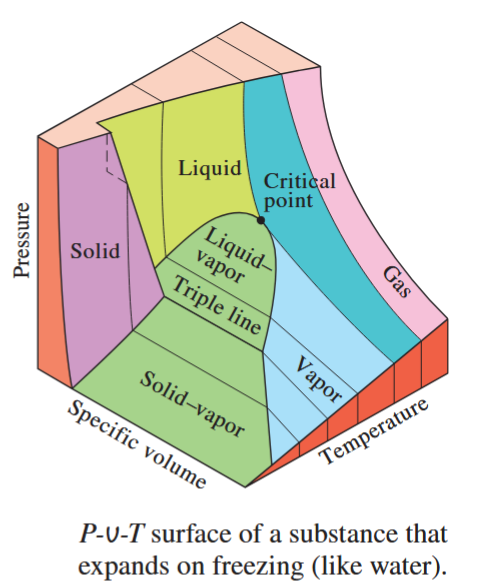
\includegraphics[width=0.35\textwidth]{PVT - Copy.png}
\end{center}
\begin{center}
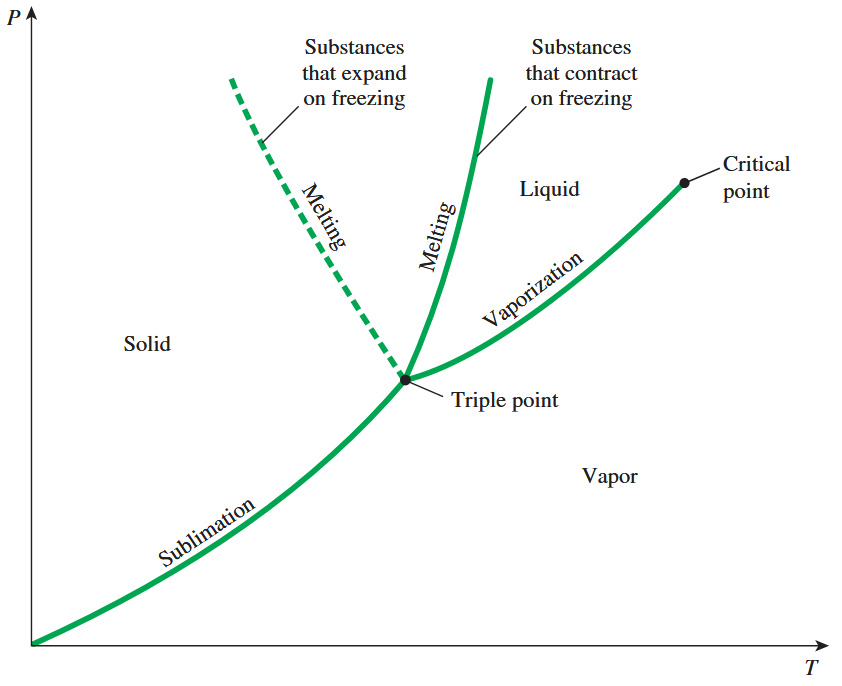
\includegraphics[width=0.5\textwidth]{../../PT.png}
\end{center}
\begin{center}
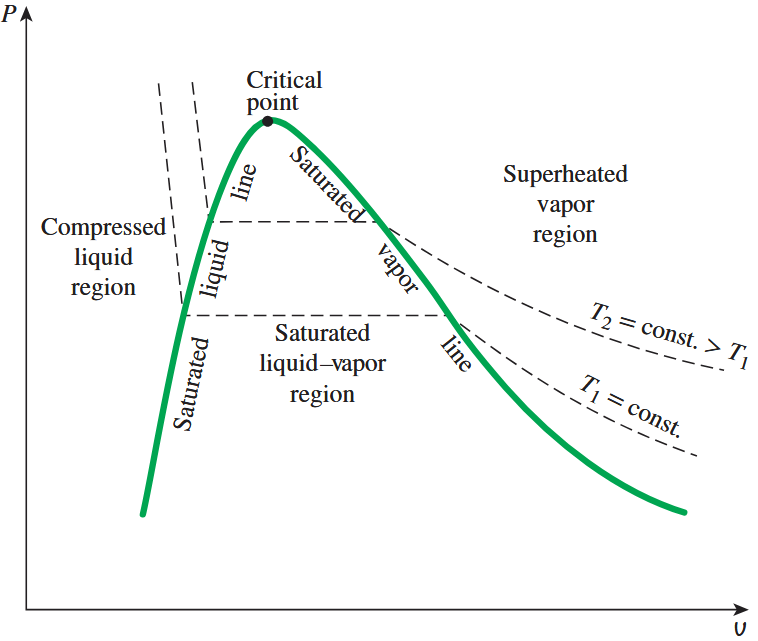
\includegraphics[width=0.5\textwidth]{../../PV.png}
\end{center}
\begin{center}
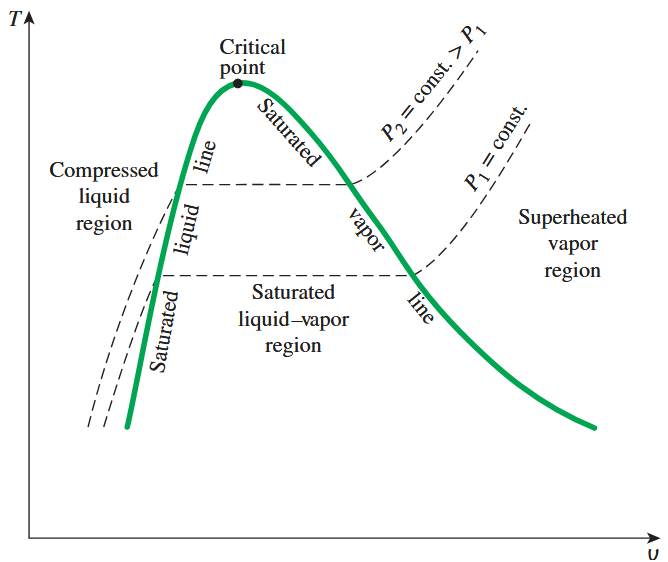
\includegraphics[width=0.5\textwidth]{../../TV.png}
\end{center}
\end{multicols}\newpage
\begin{multicols}{2}
\noindent
\textbf{Phase Change \& Saturation}\\
\hspace{-2cm}
    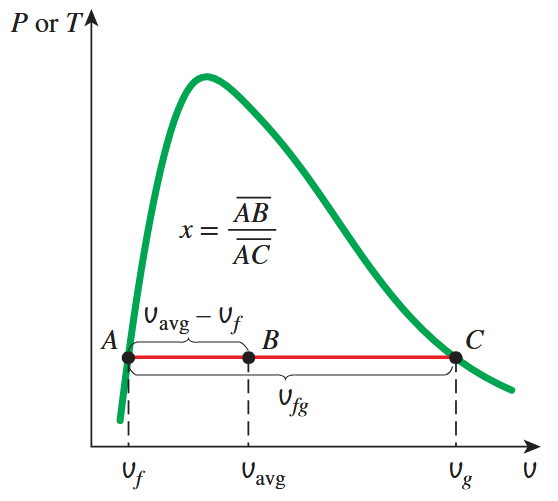
\includegraphics[width=0.35\textwidth]{../../Quality.png}\\
\[h_{fg} = h_g - h_f \quad \text{(latent heat of vaporization)}\]
\[x = \frac{m_g}{m_f + m_g} \quad \text{(quality definition)}\]
\[
\left.
\begin{aligned}
&y_{\text{avg}} = y_f + x(y_g - y_f) \quad \text{(for } \svol, h, u) \\
&x = \frac{y_{\text{avg}} - y_f}{y_g - y_f} \quad \text{(solve for quality)}
\end{aligned}
\right\} y_{fg} = y_g - y_f
\]
\textbf{Compressed Liquid Approximation}
\[y(T,P) \approx y_f(T) \quad \text{(use saturated liquid at same T)}\]
\textbf{Enthalpy}
\[h = u + P\svol,\quad \svol = \frac{1}{\rho} \quad \text{(specific enthalpy)}\]
\textbf{Specific Heat Capacity}
\[
c_{\svol} = \left(\frac{\partial u}{\partial T}\right)_{\svol} \, (\text{fixed volume})\] 
\[c_p = \left(\frac{\partial h}{\partial T}\right)_p \, (\text{fixed pressure})\]
\[\implies \Delta u = c_{\svol}\Delta T, \quad  \Delta h = c_p\Delta T \quad (\text{constant $ c_{\svol} $ or $ c_p $})
\]
\[
c_p = c_{\svol} + R \; (\text{ideal gas})\]
\[c_p = c_{\svol} \; (\text{incompressible substances})\]
\[Q = mc\Delta T \quad \text{($c_{\svol}$ or $c_p$ depending on the process)}\]
\[k=c_p/c_{\svol} \quad \text{(specific heat ratio)},  \quad c_\text{water} = 4.18 \, \frac{\text{kJ}}{\text{kg}\cdot\text{K}}\]
\textbf{Polytropic Processes}
\begin{center}
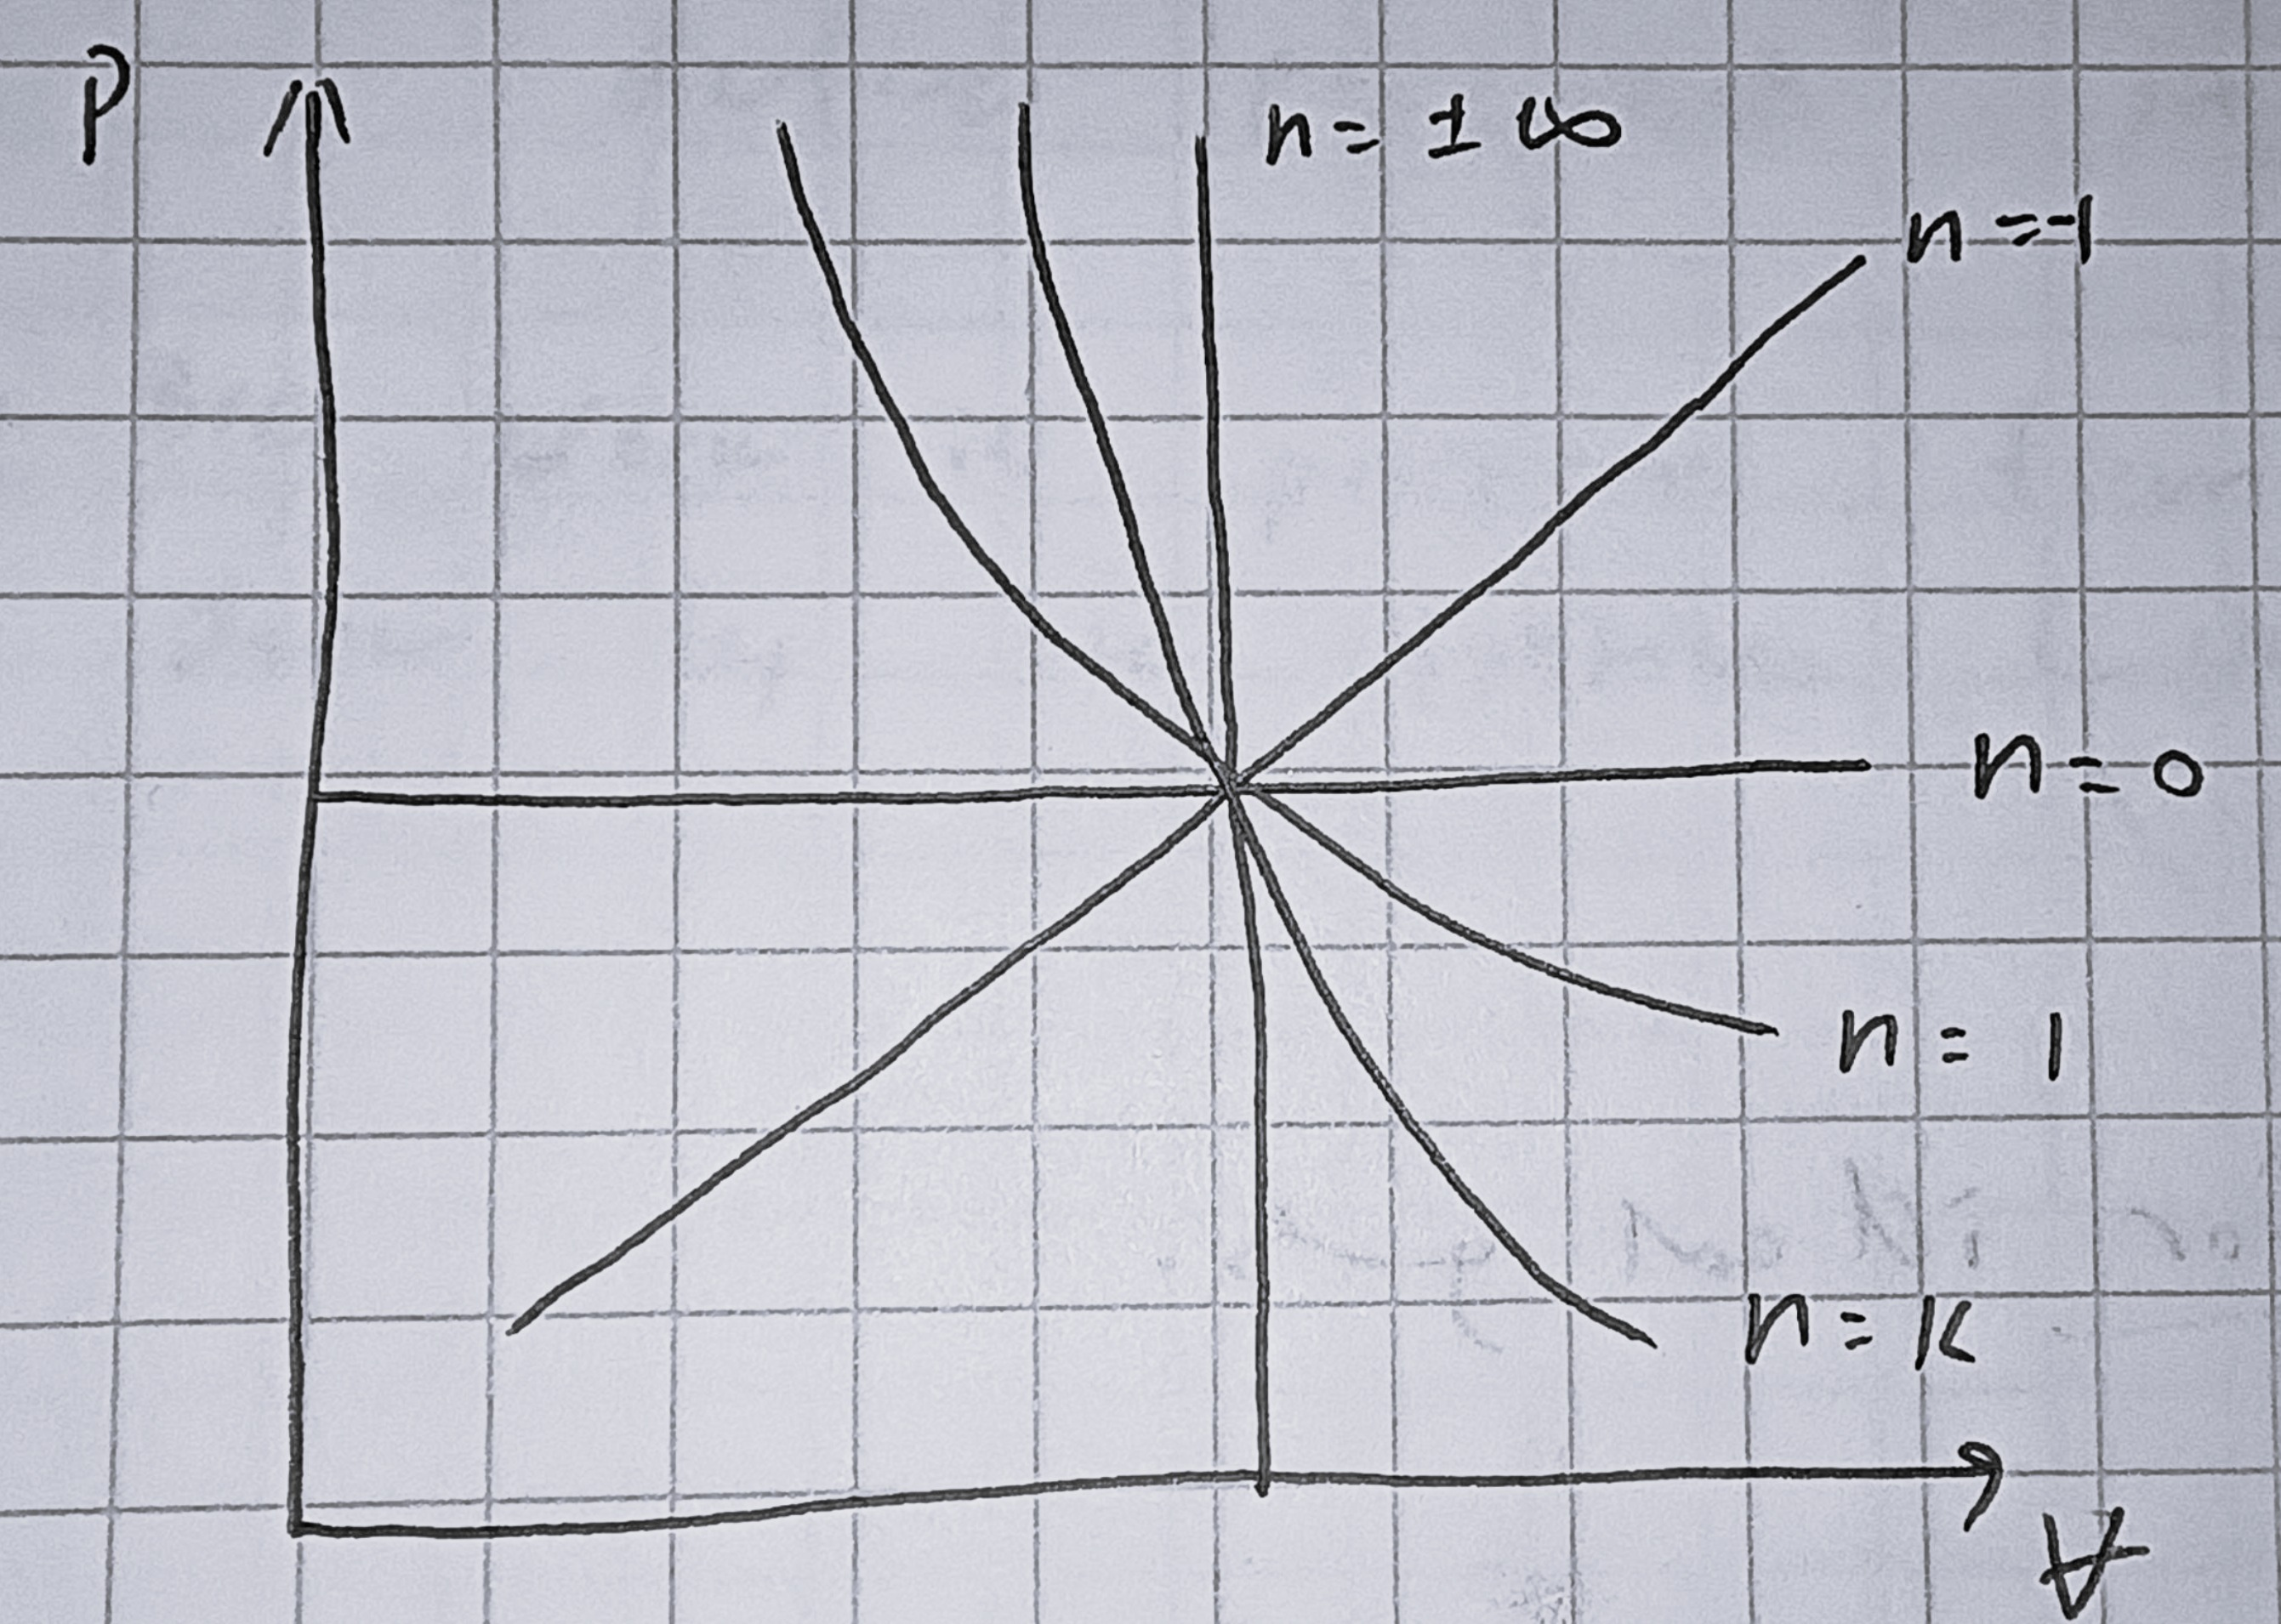
\includegraphics[width=0.4\textwidth]{Polytropic.jpg}
\end{center}
\[P\vol^n = \text{constant}\]
\begin{itemize}
    \item $n=0$: isobaric process (constant pressure)
    \item $n=1$: isothermal process (constant temperature, ideal gas)
    \item $n=k$: isentropic process (constant entropy)
    \item $n=\infty$: isochoric process (constant volume)
\end{itemize}
\newcolumn
\textbf{First Law (Closed System)}
\[\Delta U = Q - W \quad \text{(energy balance for closed system)}\]
\[\dot E_{in} - \dot E_{out} = \frac{dE_{system}}{dt} \quad \text{(rate form)}\]
\textbf{First Law (Open System)}
\[\begin{aligned}
\frac{dE}{dt} = \,&\dot{Q}-\dot{W}\\
&+
\underbrace{\sum \dot{m_i}\left[h_i+\frac{1}{2}V_i^2+g z_i\right]}_{\text{Inlet}}
-\underbrace{\sum \dot{m_e}\left[h_e+\frac{1}{2}V_e^2+g z_e\right]}_{\text{Outlet}}
\end{aligned}\]
Note:
\[\dot W = \dot m \frac{\Delta P}{\rho} = \dot \vol \Delta P \quad \text{(pump power w/ no change in KE or PE)}\]
\textbf{Mass \& Flow Relations}
\[\dot m = \rho \dot \vol = \rho A v_{avg} \quad \text{(mass flow rate)}\]
\[\dot E = \dot m e \quad \text{(energy flow rate)}\]
\textbf{Work}
\[W = \int F \cdot dx, \quad \dot{W}=F\cdot v\quad\text{(general)}\]
\[\begin{aligned}
W = \int P \,d\vol &\implies W = \frac{P_2\vol_2-P_1\vol_1}{-n+1} \quad \text{(polytropic, $n\neq1$)}\\
&\implies W = C \ln\left(\frac{\vol_2}{\vol_1}\right) \quad \text{(isothermal, $n=1$)}\\
&\implies W = P\Delta \vol \quad \text{(isobaric)}\\
\end{aligned}\]
Where $C$ is $P_1\vol_1^n = P_2\vol_2^n = C$ for a polytropic process.
\[W = \frac{1}{2}k(x_2^2 - x_1^2) \quad \text{(spring work)}\]
\textbf{Heat Transfer}
\[Q = \int \dot Q\,dt = \dot Q \Delta t \quad \text{(total heat transferred)}\]
\[\dot Q = kA \frac{\Delta T}{\Delta x} \quad \text{(conduction)}\]
\[\dot Q = hA(T_s - T_{\infty}) \quad \text{(convection)}\]
\[\dot Q = \epsilon \sigma A (T_s^4 - T_{\infty}^4) \quad \text{(radiation)}\]

\end{multicols}
\newpage
\begin{multicols}{2}
\noindent
\textbf{Efficiency}\\
\text{\scriptsize Heat engine}
\[ \eta_{HE} = \frac{W_{HE}}{Q_{H}} = \frac{Q_H-Q_L}{Q_H} \quad \leq \quad \eta_{Carnot, HE} = 1 - \frac{T_L}{T_H} \]
\text{\scriptsize Heat Pump}
\[\beta_{HP} = \frac{Q_H}{W_{HP}}=\frac{Q_H}{Q_H - Q_L} \quad \leq \quad \beta_{Carnot, HP} = \frac{T_H}{T_H - T_L} \]
\text{\scriptsize Refrigerator}
\[\beta_{Ref} = \frac{Q_L}{W_{Ref}}=\frac{Q_L}{Q_H - Q_L} \quad \leq \quad \beta_{Carnot, Ref} = \frac{T_L}{T_H - T_L} \]
\underline{Note:} The heat and work terms can also be in rate forms $\dot Q$ and $\dot W$.\\\\
$T_H$ and $T_L$ are ABSOLUTE temperatures!!\\\\
\textbf{Heat Engines}\\
Kelvin-Planck: there has to exist losses as heat to surroundings ($Q_L$).\\
Produces work from energy input as heat ($Q_H$).
\begin{center}
    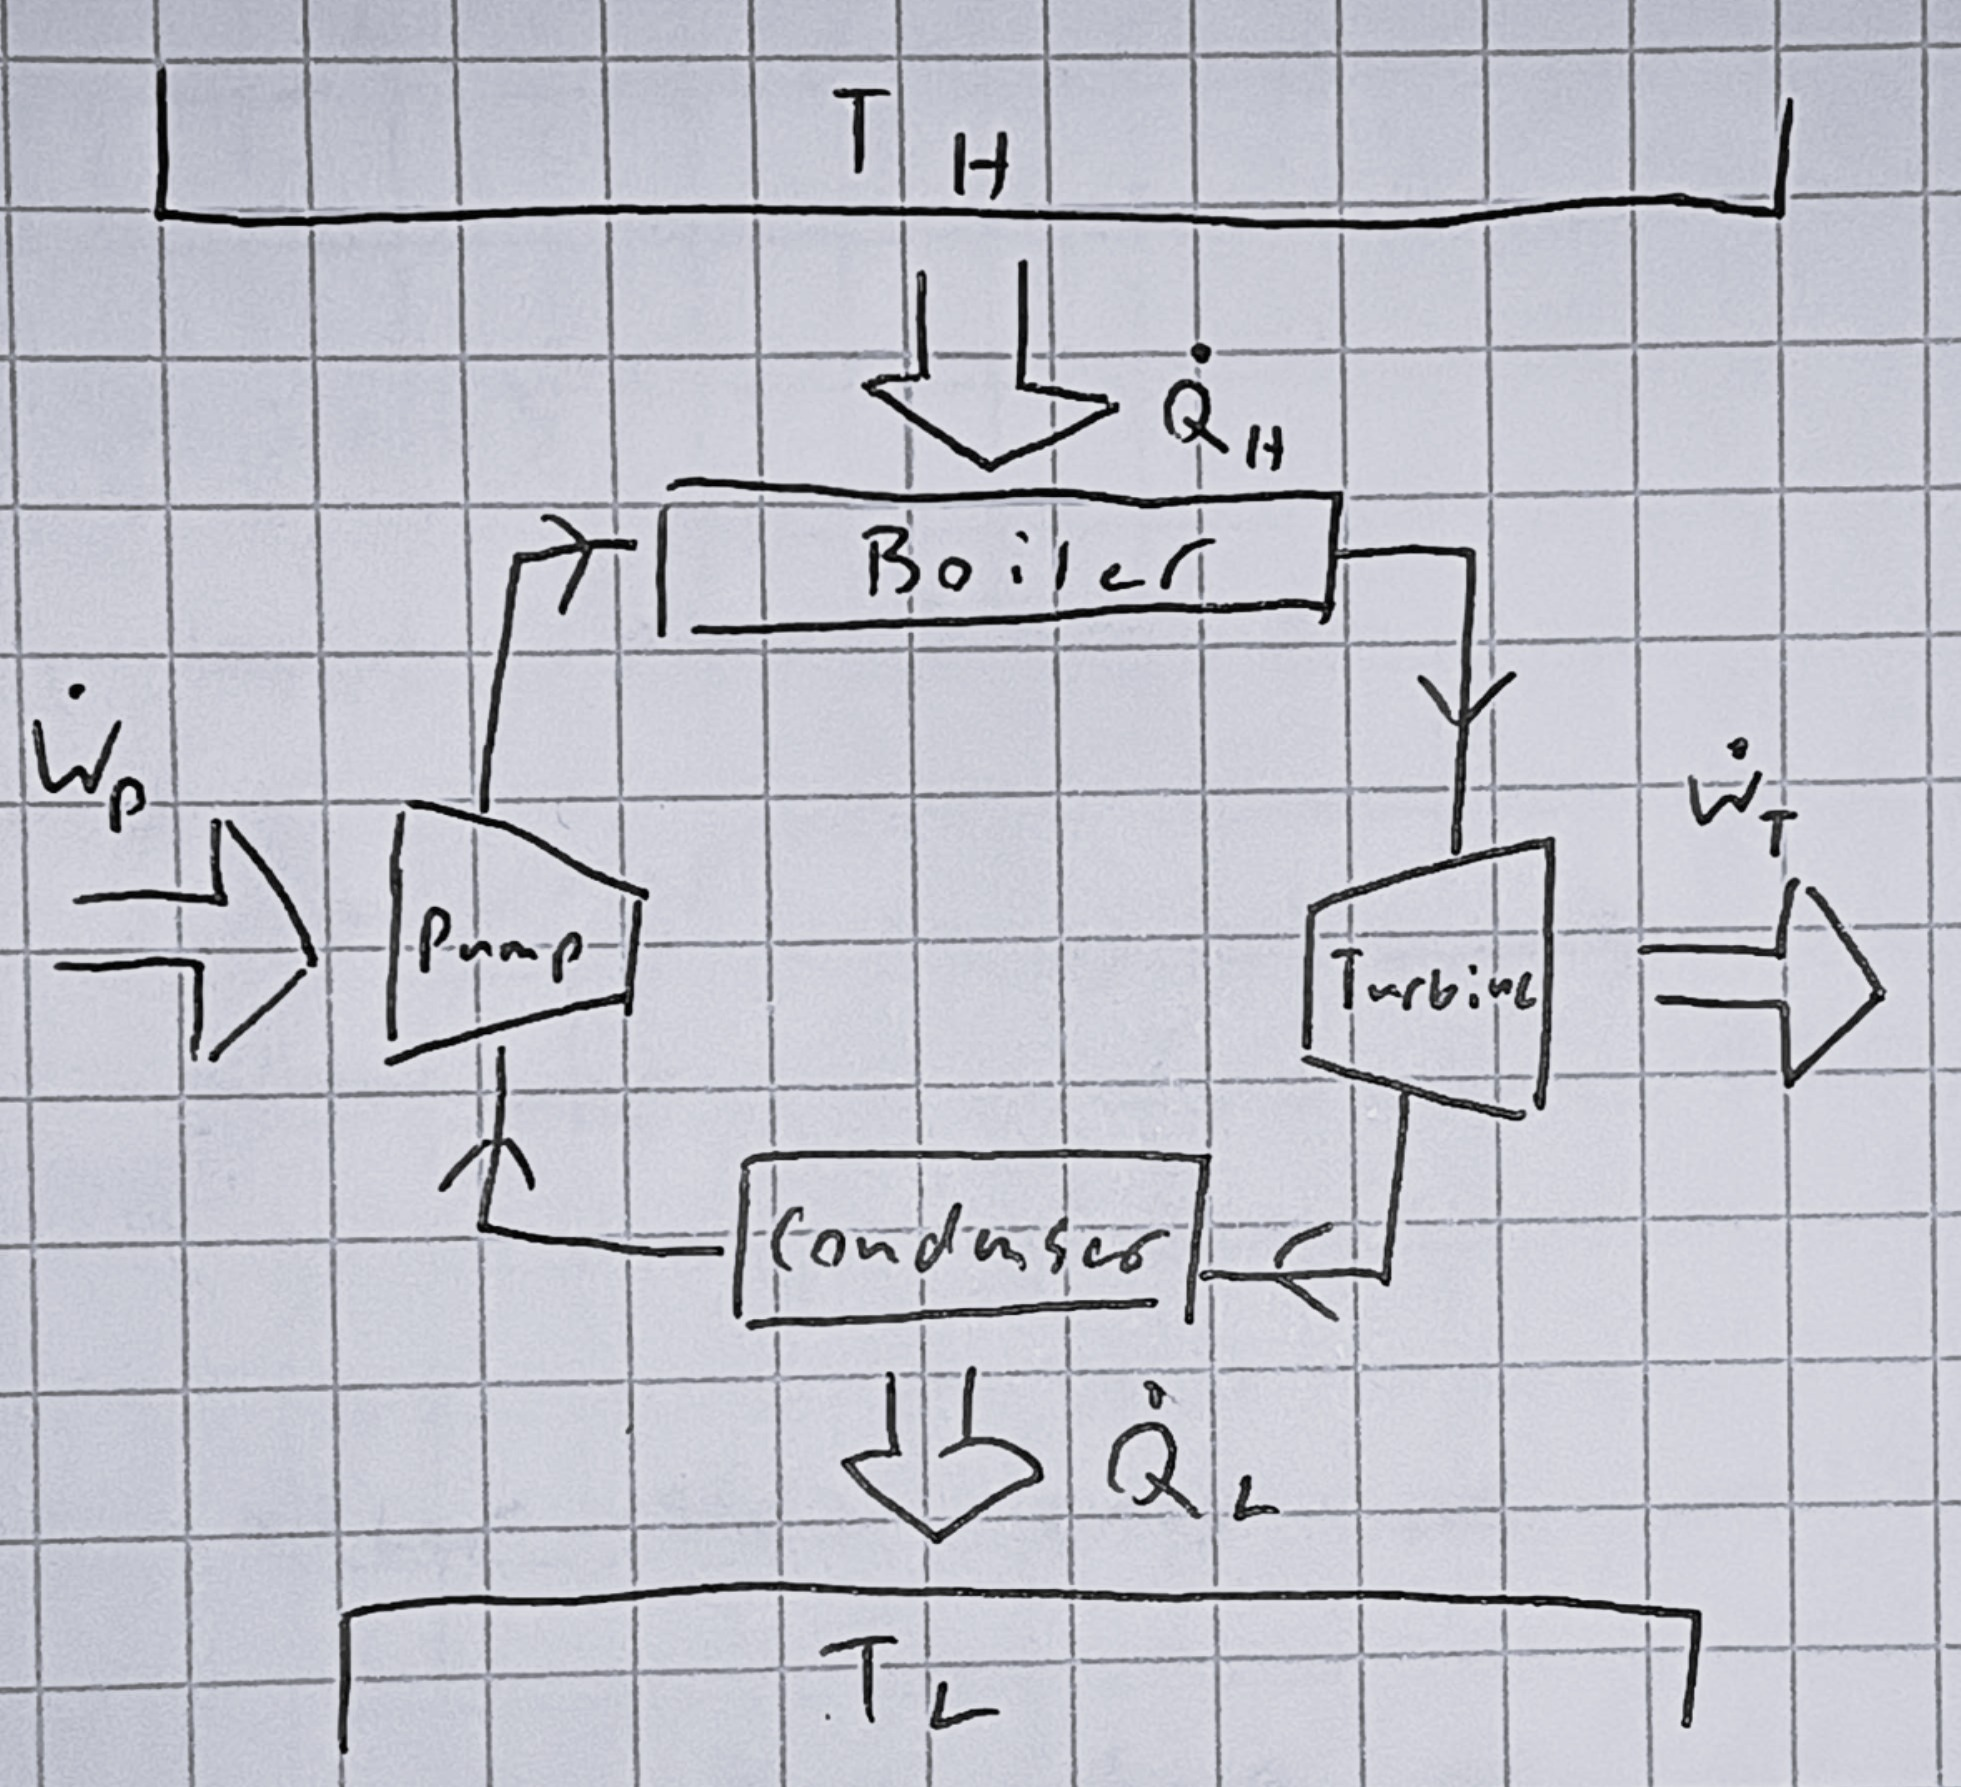
\includegraphics[width=0.4\textwidth]{HE cycle.jpg}
\end{center}
\underline{Note:} $\dot{W}_\text{net} = \dot{W}_T - \dot{W}_P$\\\\
\textbf{Refrigerators \& Heat Pumps}\\
Clausius: requires work input to transfer heat from cold to hot reservoir.\\
Refrigerators transfer heat from cold to hot reservoir, while heat pumps transfer heat from cold to hot reservoir. They have the same cycle but differ in \textit{intent}.
\begin{center}
    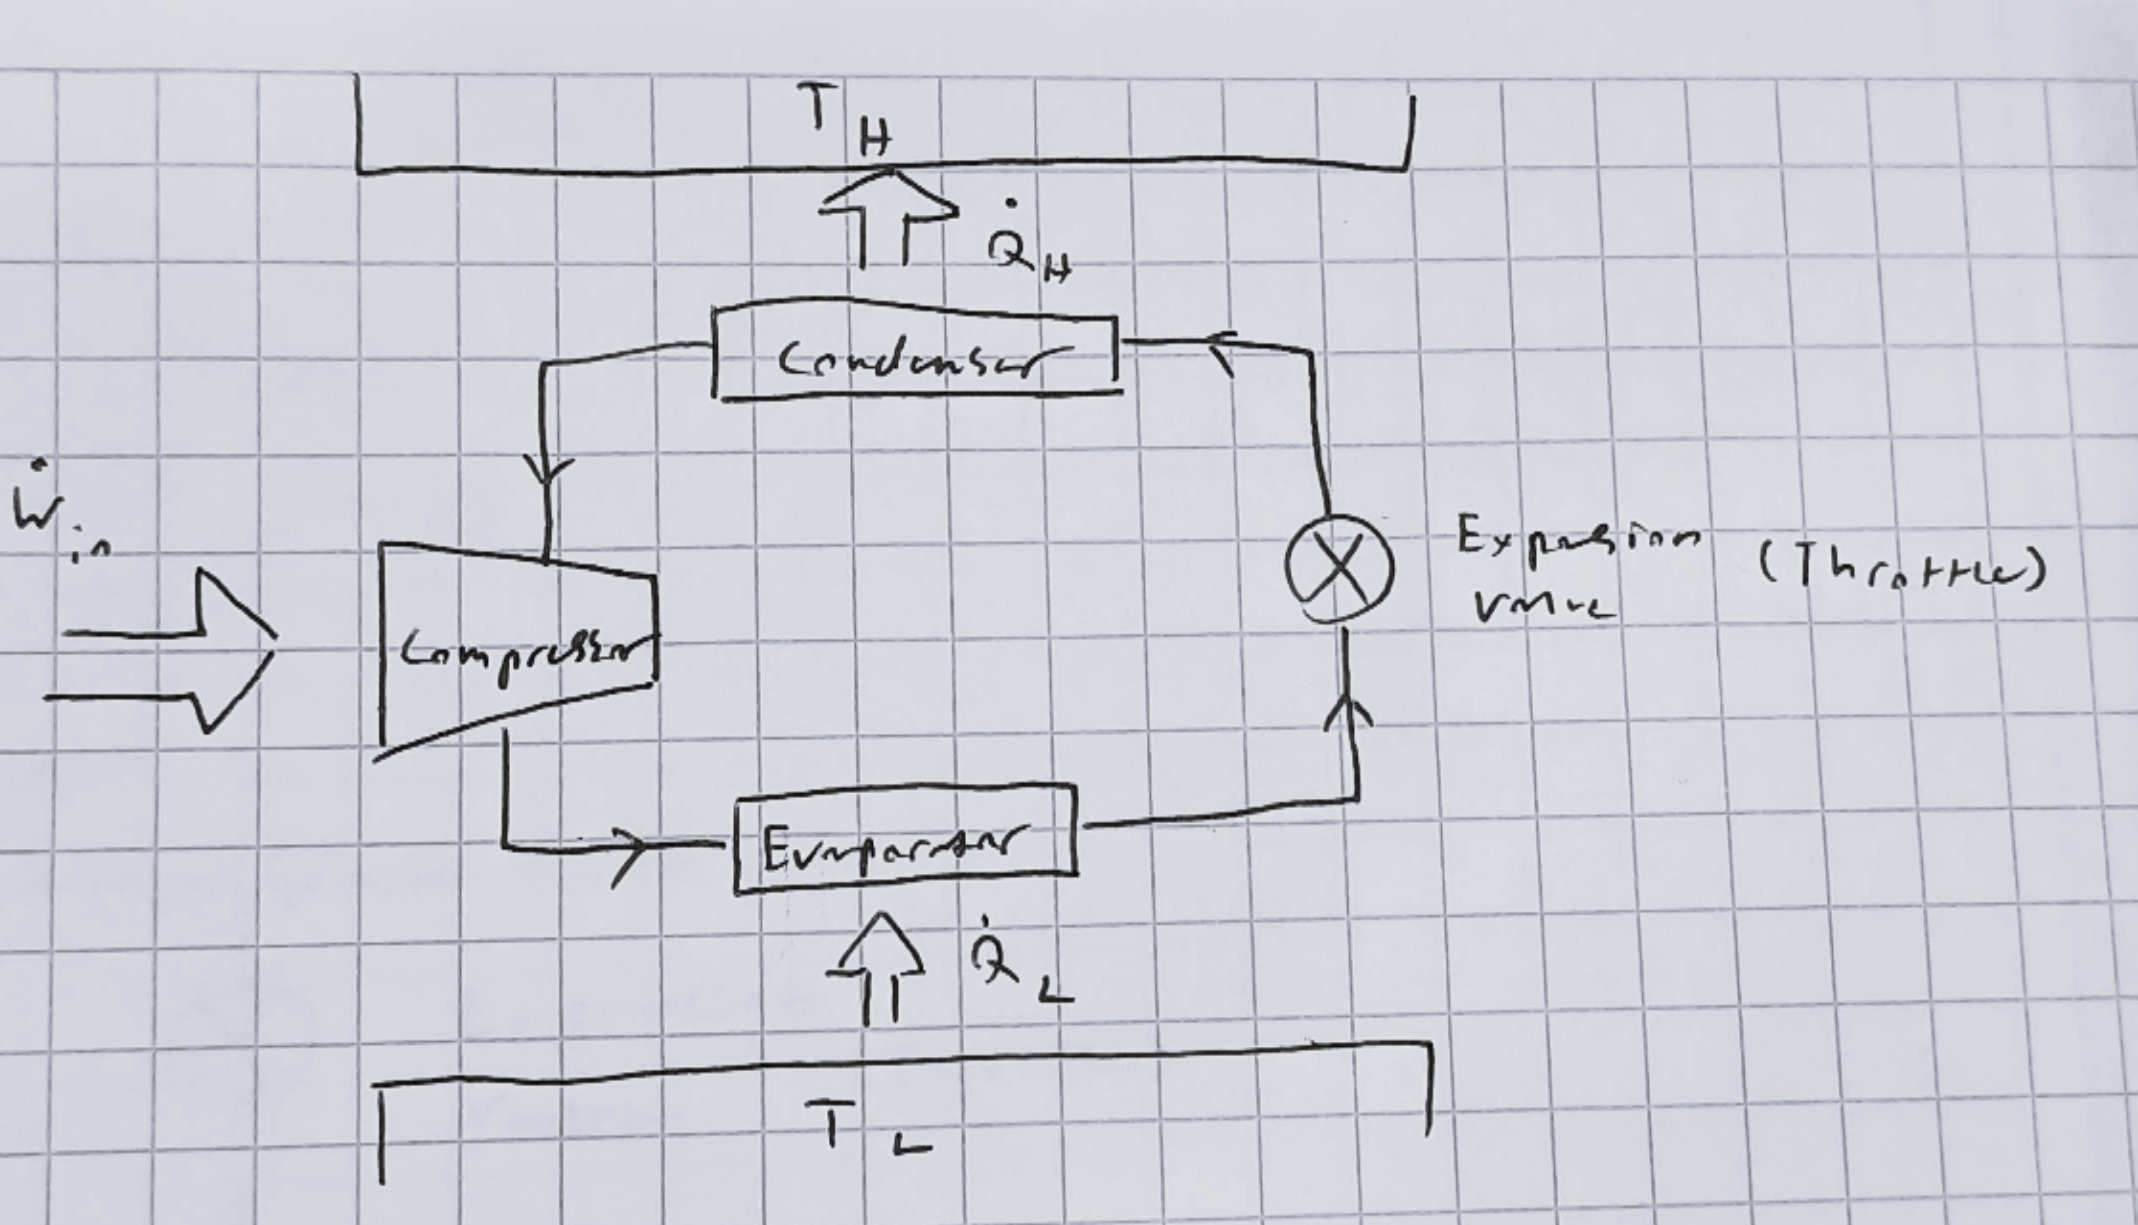
\includegraphics[width=0.5\textwidth]{Ref cycle.jpg}
\end{center}
\newcolumn
\textbf{Four Processes in a Carnot Cycle}\\
For example, in a Carnot heat engine:
\begin{itemize}
    \item $1\to2$: Reversible isothermal heat addition ($Q_H$ in at $T_H$)
    \item $2\to3$: Reversible adiabatic expansion ($T\to T_L$)
    \item $3\to4$: Reversible isothermal heat rejection ($Q_L$ out at $T_L$)
    \item $4\to1$: Reversible adiabatic compression ($T\to T_H$)
\end{itemize}
Carnot components are reversible and ideal, so they allow heat transfer even though they have no temperature difference.\\\\
All Carnot cycles operating between the same two temperature reservoirs have the same efficiency (determined by $T_H$ and $T_L$ only).\\\\
\textbf{Ideal Gas Carnot Cycle}\\
Consider the following Carnot cycle with an ideal gas in a piston-cylinder system:
\begin{center}
    
\includegraphics[width=0.35\textwidth]{ideal gas carnot.png}
\end{center}
Two isothermal processes ($dT=0$): $1\to2$ and $3\to4$\\
Two adiabatic processes ($dQ=0$): $2\to3$ and $4\to1$.\\\\
From ($P\svol = RT$), ($\delta w = Pd\svol$), and ($du =
c_{\svol}dT$):
\[\delta q = c_{\svol} dT+\frac{RT}{\svol}d\svol \quad \text{(general ODE)}\]
Integrating the ODE:
\[{}_1q_2 = RT\ln\left(\frac{\svol_2}{\svol_1}\right)\quad\text{(for an isothermal process)}\]
\[\ln\left(\frac{T_2}{T_1}\right) = -\frac{R}{c_{\svol}}\ln\left(\frac{\svol_2}{\svol_1}\right)\quad\text{(for an adiabatic process)}\]
\underline{Note:} \\For the adiabatic process, we assume a constant $c_{\svol}$, but for large temp changes, use ${c}_{\svol,\text{avg}} = (c_{\svol}(T_1)+c_{\svol}(T_2))/2$.\\\\
\textbf{Clausius Inequality}\\
For ALL cycles (reversible or irreversible):
\[\oint \frac{\delta Q}{T} \leq 0,\quad =0\text{ for reversible},\quad <0\text{ for irreversible}\]
$\oint \frac{\delta Q}{T} > 0$ is \textbf{impossible} since it violates the second law of thermodynamics
\end{multicols}
\newpage
\begin{multicols}{2}
\noindent
\textbf{Entropy Definition}\\
For a \underline{reversible process}:
\[dS \equiv \left(\frac{\delta Q}{T}\right)_\text{rev}\quad \left[\frac{\text{kJ}}{\text{K}}\right], \quad ds \equiv \left(\frac{\delta q}{T}\right)_\text{rev}\quad \left[\frac{\text{kJ}}{\text{kg$\cdot$K}}\right]\]
For a general process (reversible or irreversible):
\[S_2 - S_1 = \int_{1}^{2} \left(\frac{\delta Q}{T}\right)_\text{CS} + {}_1S_{2\text{ gen}},\quad {}_1S_{2\text{ gen}}\geq 0\]
\[\frac{dS_\text{CM}}{dt} = \frac{\dot{Q}}{T_\text{CS}}+\dot{S}_\text{gen},\quad \dot{S}_\text{gen}\geq 0\]
$Q$ refers to the heat transfer across the system boundary and $T_\text{CS}$ is the temperature at the system boundary where the heat transfer occurs.\\\\
\textbf{T-S Plots}\\
\begin{center}
    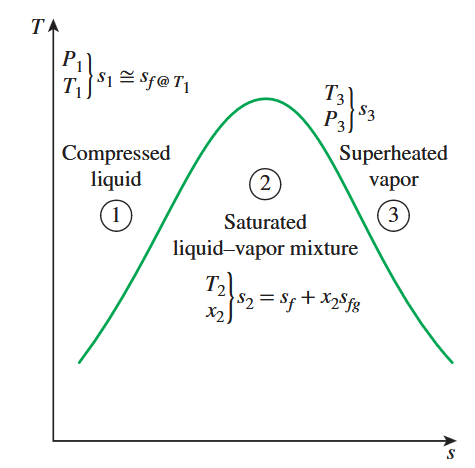
\includegraphics[width=0.4\textwidth]{entropy property.png}
\end{center}
\begin{center}
    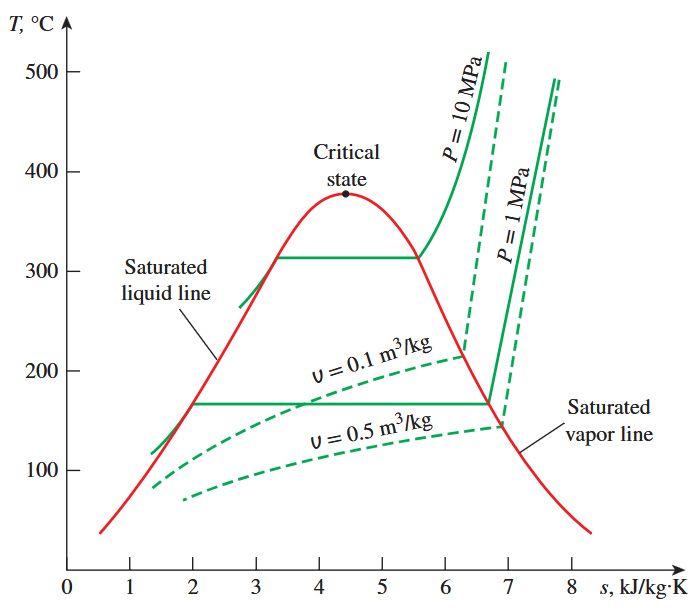
\includegraphics[width=0.5\textwidth]{TS more like tspmo.png}
\end{center}
\textbf{Heat Transfer for a Reversible Process}
\[Q = \int TdS\quad \text{(area under the T-S plot)}\]
\textbf{Entropy Change for a Phase Change}
\[s_\text{fg} = \frac{h_\text{fg}}{T_\text{sat}}\]
\newcolumn\\
\textbf{Carnot Cycle (Reversible) on T-S Plots}
\begin{center}
    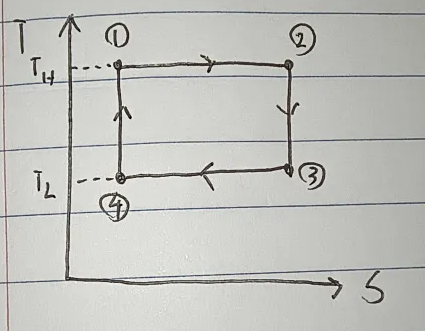
\includegraphics[width=0.35\textwidth]{carnot TS.png}
\end{center}
Isothermal processes are horizontal lines, and adiabatic processes are isentropic (vertical) lines (since $dS = \delta Q/T = 0$ for reversible adiabatic processes).\\\\
\textbf{Gibbs Relations}\\
General thermodynamic relationships between entropy and other properties:
\[Tds = du + Pd\svol\quad \text{(First Gibbs Relation)}\]
\[Tds = dh - \svol dP\quad \text{(Second Gibbs Relation)}\]
\textbf{Gibbs Relations for Ideal Gas}\\
From First Gibbs Relation:
\[ds =\frac{C_{\svol0}}{T}dT+\frac{R}{\svol}d\svol\]
\[\implies s_2-s_1 = C_{\svol0}\ln\left(\frac{T_2}{T_1}\right)+R \ln\left(\frac{\svol_2}{\svol_1}\right)\]
From Second Gibbs Relation:
\[ds = \frac{C_{P0}}{T}dT-\frac{R}{P}dP\]
\[\implies s_2-s_1 = C_{P0}\ln\left(\frac{T_2}{T_1}\right)-R \ln\left(\frac{P_2}{P_1}\right)\]
Note that these two equations are equivalent since $C_{P0} = C_{\svol0} + R$ for an ideal gas.\\\\
\textbf{Isentropic Relations for Ideal Gases} ($P\vol^k = \text{constant}$)
\[\frac{T_2}{T_1} = \left(\frac{P_2}{P_1}\right)^{\frac{k-1}{k}}, \quad \frac{T_2}{T_1} = \left(\frac{\vol_1}{\vol_2}\right)^{k-1},\quad \frac{P_2}{P_1} = \left(\frac{\vol_1}{\vol_2}\right)^k\]
\textbf{Entropy Balance}\\
For a CLOSED system:
\[\sum \frac{Q_k}{T_k}+S_{\text{gen}}=\Delta S_{\text{sys}} \quad [\text{kJ/K}]\]
For an OPEN system:
\[\sum \frac{\dot{Q}_k}{T_k} +\sum \dot{m}_i s_i - \sum \dot{m}_e s_e + \dot{S}_\text{gen} = \frac{dS_\text{CV}}{dt} \quad [\text{kW/K}]\]

\end{multicols}









\end{document}
